\begin{pastexam}[label={px:df3-108-ds-03}]{地方三等資訊處理 108 年 第三題}
（申論；20 分）

下圖為一棵 2-3-4 樹。
\begin{itemize}[leftmargin=2.2em]
\item[㈠] 請畫出對應的紅黑樹（red-black tree）。請參閱上題紅黑樹節點的標示說明。（6 分）
\item[㈡] 首先，插入（insert）33；接著，刪去（delete）78。請分別畫出對應的 2-3-4 樹與紅黑樹。（14 分）
\end{itemize}
\begin{center}
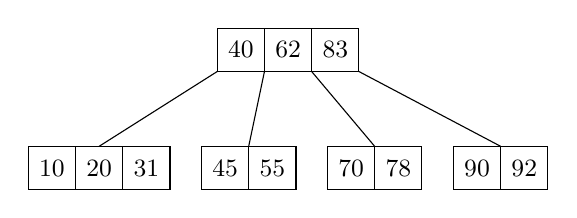
\begin{tikzpicture}[k/.style={draw,minimum width=6mm,minimum height=5.5mm,inner sep=0pt,font=\small}]
\foreach \v/\x in {40/2.4, 62/3.0, 83/3.6} \node[k] at (\x,0) {\v};
\foreach \v/\x in {10/0, 20/0.6, 31/1.2, 45/2.2, 55/2.8, 70/3.8, 78/4.4, 90/5.4, 92/6.0} \node[k] at (\x,-1.5) {\v};
\draw (2.1,-0.275) -- (0.6,-1.225);
\draw (2.7,-0.275) -- (2.5,-1.225);
\draw (3.3,-0.275) -- (4.1,-1.225);
\draw (3.9,-0.275) -- (5.7,-1.225);
\end{tikzpicture}
\end{center}
（「上題」指本卷第二題：紅節點標示 R，例如 20R；黑節點標示 B，例如 50B。）
\end{pastexam}

\begin{pastsoln}
2-3-4 樹和紅黑樹的對應見資結書第~10.4~節、第~11.1~節：2-節點 $\{a\}$ 是一個黑節點；3-節點 $\{a, b\}$ 是黑的
$a$ 加紅的右子 $b$（或黑的 $b$ 加紅的左子 $a$，兩種都可以）；4-節點 $\{a, b, c\}$ 是黑的 $b$ 加兩個紅子
$a$、$c$。 下面的 3-節點一律用「黑的小鍵、紅的右子是大鍵」。

\textbf{㈠} 逐個節點轉換：
\begin{itemize}
\item 根 $[40\ 62\ 83]$ 是 4-節點：$62$B，左子 $40$R、右子 $83$R。
\item $[10\ 20\ 31]$ 是 4-節點：$20$B，左右子 $10$R、$31$R，接在 $40$ 的左邊。
\item $[45\ 55]$：$45$B 加右子 $55$R，接在 $40$ 的右邊（$40 < 45, 55 < 62$）。
\item $[70\ 78]$：$70$B 加右子 $78$R，接在 $83$ 的左邊。
\item $[90\ 92]$：$90$B 加右子 $92$R，接在 $83$ 的右邊。
\end{itemize}
\begin{center}
\begin{tikzpicture}[every node/.style={ellipse,draw,minimum height=6mm,minimum width=9mm,inner sep=1pt,font=\small},
  bk/.style={fill=black,text=white}, rd/.style={draw=red!70!black,very thick,fill=red!12},
  level distance=10mm, level 1/.style={sibling distance=48mm}, level 2/.style={sibling distance=24mm},
  level 3/.style={sibling distance=12mm}]
\node[bk] {62B}
  child {node[rd] {40R}
    child {node[bk] {20B} child {node[rd] {10R}} child {node[rd] {31R}}}
    child {node[bk] {45B} child[missing] child {node[rd] {55R}}}}
  child {node[rd] {83R}
    child {node[bk] {70B} child[missing] child {node[rd] {78R}}}
    child {node[bk] {90B} child[missing] child {node[rd] {92R}}}};
\end{tikzpicture}
\end{center}
（黑底白字是黑節點，粗框淺底是紅節點。） 檢查：紅節點的子節點都是黑的；根到每個空指標都經過 $2$ 個黑節點
（含根），等於 2-3-4 樹的層數。 若 3-節點改用另一種排法（例如 $55$B 帶左子 $45$R），也是正確答案。

\textbf{㈡ 插入 33。}

\textbf{2-3-4 樹}：用資結書虛擬碼~11.1 由上而下的插入，往下走的路上遇到 4-節點就先分裂。
\begin{enumerate}
\item 根 $[40\ 62\ 83]$ 是 4-節點，先分裂：$62$ 成為新的根，$[40]$、$[83]$ 是它的兩個子節點，原來的四個子
節點分給它們。 樹長高一層。
\item $33 < 62$，往 $[40]$ 走；$33 < 40$，下一個是 $[10\ 20\ 31]$，是 4-節點，先分裂：$20$ 上到父節點成
$[20\ 40]$，剩下 $[10]$、$[31]$。
\item $33 > 20$ 且 $< 40$，走到 $[31]$，是葉子，放進去成 $[31\ 33]$。
\end{enumerate}

\textbf{紅黑樹}：在㈠的紅黑樹上用資結書虛擬碼~10.6 插入 $33$：$62 \to 40 \to 20 \to 31$，成為 $31$ 的右子（紅）。
父 $31$ 紅、叔叔 $10$ 紅，情況 1：$31$、$10$ 改黑，$20$ 改紅；$z$ 移到 $20$，父 $40$ 紅、叔叔 $83$ 紅，再一次
情況 1：$40$、$83$ 改黑，$62$ 改紅；$62$ 是根，塗回黑。 兩次改色正好對應 2-3-4 樹的兩次分裂，黑高度加一
對應樹長高一層。

\textbf{㈡ 接著刪去 78。}

\textbf{2-3-4 樹}：$78$ 在葉子 $[70\ 78]$ 裡，刪掉後剩 $[70]$，仍有一個鍵，不必借或合併。

\textbf{紅黑樹}：$78$R 是沒有子節點的紅葉子，直接拿掉；刪掉紅節點不改變任何路徑上的黑節點數，不必修正
（資結書虛擬碼~10.7）。

結果如下，先是兩棵 2-3-4 樹（左：插入 33 之後；右：再刪去 78 之後），再是對應的兩棵紅黑樹：
\begin{center}
\begin{tikzpicture}[k/.style={draw,minimum width=6mm,minimum height=5.5mm,inner sep=0pt,font=\small},
  lab/.style={font=\small}]
\node[k] at (3.4,0) {62};
\node[k] at (1.3,-1.3) {20}; \node[k] at (1.9,-1.3) {40};
\node[k] at (5.5,-1.3) {83};
\foreach \v/\x in {10/0, 31/1.0, 33/1.6, 45/2.6, 55/3.2, 70/4.4, 78/5.0, 90/6.0, 92/6.6} \node[k] at (\x,-2.6) {\v};
\draw (3.1,-0.275) -- (1.6,-1.025);
\draw (3.7,-0.275) -- (5.5,-1.025);
\draw (1.0,-1.575) -- (0,-2.325);
\draw (1.6,-1.575) -- (1.3,-2.325);
\draw (2.2,-1.575) -- (2.9,-2.325);
\draw (5.2,-1.575) -- (4.7,-2.325);
\draw (5.8,-1.575) -- (6.3,-2.325);
\node[lab] at (3.3,-3.3) {插入 33 之後};
\begin{scope}[xshift=80mm]
\node[k] at (3.4,0) {62};
\node[k] at (1.3,-1.3) {20}; \node[k] at (1.9,-1.3) {40};
\node[k] at (5.5,-1.3) {83};
\foreach \v/\x in {10/0, 31/1.0, 33/1.6, 45/2.6, 55/3.2, 70/4.7, 90/6.0, 92/6.6} \node[k] at (\x,-2.6) {\v};
\draw (3.1,-0.275) -- (1.6,-1.025);
\draw (3.7,-0.275) -- (5.5,-1.025);
\draw (1.0,-1.575) -- (0,-2.325);
\draw (1.6,-1.575) -- (1.3,-2.325);
\draw (2.2,-1.575) -- (2.9,-2.325);
\draw (5.2,-1.575) -- (4.7,-2.325);
\draw (5.8,-1.575) -- (6.3,-2.325);
\node[lab] at (3.3,-3.3) {再刪去 78 之後};
\end{scope}
\end{tikzpicture}

\medskip
\begin{tikzpicture}[every node/.style={ellipse,draw,minimum height=6mm,minimum width=9mm,inner sep=1pt,font=\small},
  bk/.style={fill=black,text=white}, rd/.style={draw=red!70!black,very thick,fill=red!12},
  lab/.style={draw=none,fill=none,font=\small},
  level distance=10mm, level 1/.style={sibling distance=48mm}, level 2/.style={sibling distance=24mm},
  level 3/.style={sibling distance=15mm}, level 4/.style={sibling distance=10mm}]
\node[bk] {62B}
  child {node[bk] {40B}
    child {node[rd] {20R} child {node[bk] {10B}} child {node[bk] {31B} child[missing] child {node[rd] {33R}}}}
    child {node[bk] {45B} child[missing] child {node[rd] {55R}}}}
  child {node[bk] {83B}
    child {node[bk] {70B} child[missing] child {node[rd] {78R}}}
    child {node[bk] {90B} child[missing] child {node[rd] {92R}}}};
\node[lab] at (0,-4.6) {插入 33 之後};
\begin{scope}[yshift=-55mm]
\node[bk] {62B}
  child {node[bk] {40B}
    child {node[rd] {20R} child {node[bk] {10B}} child {node[bk] {31B} child[missing] child {node[rd] {33R}}}}
    child {node[bk] {45B} child[missing] child {node[rd] {55R}}}}
  child {node[bk] {83B}
    child {node[bk] {70B}}
    child {node[bk] {90B} child[missing] child {node[rd] {92R}}}};
\node[lab] at (0,-4.6) {再刪去 78 之後};
\end{scope}
\end{tikzpicture}
\end{center}
檢查紅黑樹：根到每個空指標都經過 $3$ 個黑節點（含根），例如 $62 \to 40 \to 20 \to 10$、
$62 \to 40 \to 20 \to 31 \to 33$、$62 \to 83 \to 70$；沒有紅節點接紅節點。 把每個黑節點和它的紅子節點合起來，
正好得到前面的 2-3-4 樹：$[62]$；$[20\ 40]$、$[83]$；$[10]$、$[31\ 33]$、$[45\ 55]$、$[70\ 78]$（刪後 $[70]$）、
$[90\ 92]$。
\end{pastsoln}
